\documentclass[]{article}
\usepackage[a4paper, total={15cm,23cm}]{geometry}
\usepackage{fancyhdr}
\usepackage{graphicx}
\usepackage{amsmath}
\usepackage{amssymb}
\usepackage{xcolor}
\usepackage{verbatim}
%opening
\title{PH 222 Activity 9}
\author{Benjamin Bauml}
\date{Winter 2021}
\pagestyle{fancy}
\rhead{PH 222}
\chead{Winter 2021}
\lhead{Activity 9}

%Custom Quotation Command
\newcommand{\excerpt}[1]{\colorbox{lightgray}{\parbox{14.8cm}{#1}} \\}

\begin{document}

\maketitle

\begin{center}
These problems are borrowed/adapted from Chapter 34 of \textit{Physics for Scientists and Engineers}, as well as its associated \textit{Student Workbook}.
\end{center}
\section*{Activity 1}%WB3
\excerpt{
Are the following most reasonably described by the wave model of light, the ray model of light, either, or neither?
}
%\begin{comment}%comment out this comment environment when revealing solutions
\begin{center}
	\begin{tabular}{c|c}
		Situation & Model \\
		\hline\hline
		human eye & \\
		\hline
		optical telescope & \\
		\hline
		antireflection coatings on the telescope lenses & \\
		\hline
		light passing through a 1-cm-diameter hole & \\
		\hline
		light passing through a 0.1-mm-diameter hole & \\
		\hline
		interferometer & \\
		\hline
		white light dispersed into a rainbow by a prism & \\
		\hline
		white light dispersed into a rainbow by a diffraction grating & \\
	\end{tabular}
\end{center}
%\end{comment}
\begin{comment}%uncomment this comment environment when revealing solutions
\begin{center}
	\begin{tabular}{c|c}
		Situation & Model \\
		\hline\hline
		human eye & ray \\
		\hline
		optical telescope & ray \\
		\hline
		antireflection coatings on the telescope lenses & wave \\
		\hline
		light passing through a 1-cm-diameter hole & ray \\
		\hline
		light passing through a 0.1-mm-diameter hole & wave \\
		\hline
		interferometer & wave \\
		\hline
		white light dispersed into a rainbow by a prism & ray \\
		\hline
		white light dispersed into a rainbow by a diffraction grating & wave \\
	\end{tabular}
\end{center}
\end{comment}

\section*{Activity 2}%WB11
\excerpt{
Draw seven rays from the object that refract after passing through the seven dots on the boundary.
}
\begin{center}
	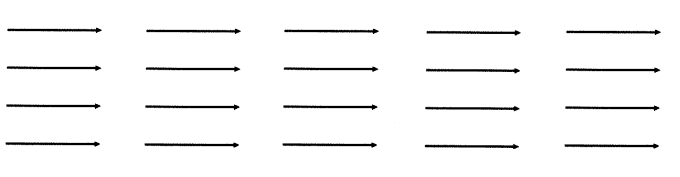
\includegraphics[scale=0.5]{A2}
	%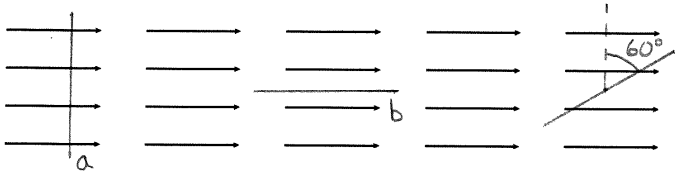
\includegraphics[scale=0.5]{A2Sol}%Solution
\end{center}

\pagebreak
\section*{Activity 3}%WB23
\excerpt{
An object is near a lens whose focal points are shown.
}
\excerpt{
(a) Use ray tracing to locate the image of this object.
}
\begin{center}
	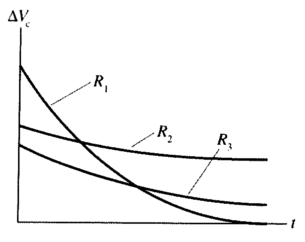
\includegraphics[scale=0.5]{A3}
	%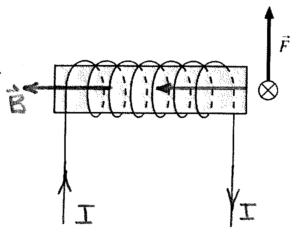
\includegraphics[scale=0.5]{A3Sol}%Solution
\end{center}
\excerpt{
(b) Is the image upright or inverted?
}
% To reveal the solution, delete "\phantom{\parbox{\textwidth}{" from the beginning, and "}}" from the end.
\phantom{\parbox{\textwidth}{
Upright \\
}}
\excerpt{
(c) Is the image height larger or smaller than the object height?
}
% To reveal the solution, delete "\phantom{\parbox{\textwidth}{" from the beginning, and "}}" from the end.
\phantom{\parbox{\textwidth}{
Larger \\
}}
\excerpt{
(d) Is this a real or a virtual image? Explain how you can tell.
}
% To reveal the solution, delete "\phantom{\parbox{\textwidth}{" from the beginning, and "}}" from the end.
\phantom{\parbox{\textwidth}{
Virtual. The rays do not converge on the image point. Instead, the rays \underline{appear} to diverge from the image point. \\
}}
\excerpt{
(e) Say you are given that the object is a distance $ \frac{2f}{3} $ from the lens (where $ f $ is the focal length). How far back is the image, and how does its height compare to that of the object?
}
% To reveal the solution, delete "\phantom{\parbox{\textwidth}{" from the beginning, and "}}" from the end.
\phantom{\parbox{\textwidth}{
In other words, $ s = \frac{2f}{3} $. By the thin lens equation,
\[
\begin{split}
	\frac{1}{s} + \frac{1}{s'} & = \frac{1}{f} \\
	\frac{3}{2f} + \frac{1}{s'} & = \frac{1}{f} \\
	\frac{1}{s'} & = -\frac{1}{2f} \\
	s' & = -2f.
\end{split}
\]
The negative sign suggests a virtual image, which is a distance $ 2f $ from the lens on the same side as the object. The magnification is
\[
m = -\frac{s'}{s} = \frac{2f}{2f/3} = 3,
\]
and the height ratio $ h'/h = |m| = 3 $, so the image is 3 times as tall as the object.
}}

\pagebreak
\section*{Activity 4}%TB34.13
\excerpt{
An underwater diver sees the sun 50$ ^{\circ} $ above horizontal. How high is the sun above the horizon to a fisherman in a boat above the diver?
}
% To reveal the solution, delete "\phantom{\parbox{\textwidth}{" from the beginning, and "}}" from the end.
\phantom{\parbox{\textwidth}{
\begin{center}
	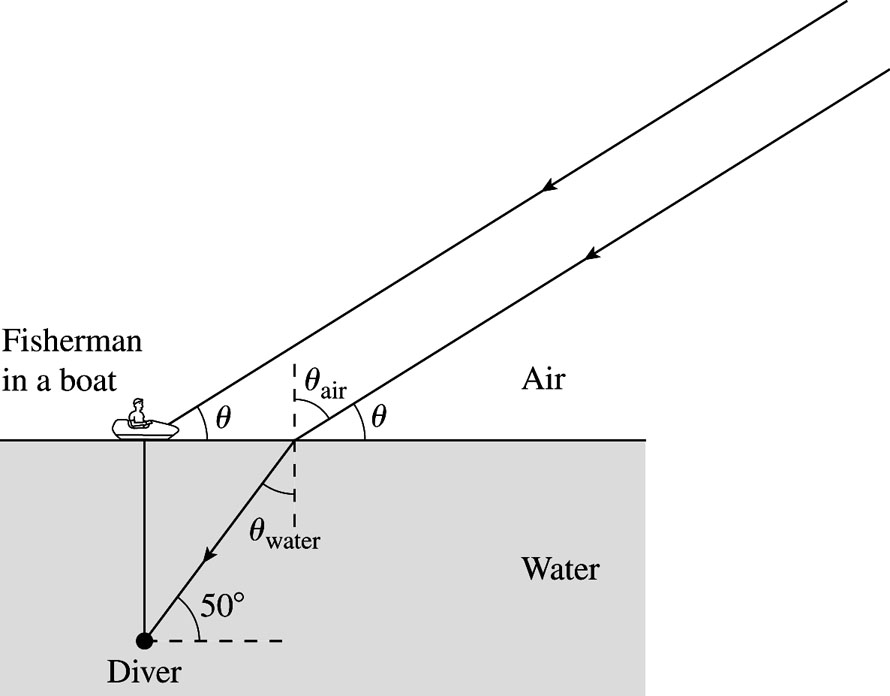
\includegraphics[scale=0.2]{BoatDiver}
\end{center}
The angle the diver sees the sun at is part of a right triangle, with the angle the incoming ray makes with the vertical ($ \theta_{water} $) being the other non-right angle. As such, $ \theta_{water} = 40^{\circ} $. \\
\indent We can relate $ \theta_{water} $ to $ \theta_{air} $ by Snell's law:
\[
n_{air}\sin\theta_{air} = n_{water}\sin\theta_{water} \implies \sin\theta_{air} = \frac{n_{water}}{n_{air}}\sin\theta_{water} = \frac{1.33}{1.0}\sin(40^{\circ})\implies \theta_{air} \approx 58.7^{\circ}.
\]
The angle above the horizon is complementary to this angle, so $ \theta = 90^{\circ}-\theta_{air} = 31.3^{\circ} \approx 31^{\circ} $. Since the sun is far away from both the fisherman and the diver, its rays are parallel, so the fisherman will see the sun at the same angle above the horizon.
}}


\end{document}